% !TEX root = ../thesis-example.tex
%
\chapter{Geste instumental}
\label{ch:gesture}

\cleanchapterquote{La percussion de ce pseudo-gong est illlusoire : rien ne tape sur rien dans l’ordinateur. Schumann qualifiait le legato au piano de ``trompe-l’oreille'' : la musique est aussi un art du mirage, de l’illusion.}{Jean-Claude Risset}{Discours invité aux JIM 2010 \cite{risset_propos_2010}}


\noindent Poursuivant des évolutions organologiques latentes, telles que présentées dans la section \ref{sec:ephemerality:landscape}, les \glspl{DMI} finissent d'opérer un découplage énergétique, une ``dislocation du controle'' (\textit{control dislocation} \cite{miranda_new_2006}), rompant avec plus de 40.000 ans de tradition musicale \cite{conard_new_2009} et avec l'unité de temps, de lieu et d'action —définie en règle par le théâtre classique, mais qui reflète la relation qui existait entre l'auditeur et le phénomène sonore, comme le rappelle Genevois dans \cite{cance_what_2012}. Nous allons voir dans ce chapitre comment le geste instrumental s'en trouve affecté, par un examen critique des catégories gestuelles déjà proposées, et la proposition de nouvelles catégories prenant en compte l'aspect subversif de l'art musical.


\section{Introduction}

\subsection{Définition}

Le Littré, le Larousse ou le dictionnaire de l'Académie Française s'accordent à définir le geste comme ``un mouvement du corps, principalement de la main, des bras, de la tête, porteur de sens ou non'' (Larousse).

Les études du geste musical et du geste instrumental s'accordent, elle, à le définir comme l'association d'un mouvement et d'une intention. 
\iquote{Le geste doit être défini comme un mouvement intentionnel plus ou moins complexe, orienté vers un but déterminé qui lui donne un sens individuel, social ou historique.} \cite{imberty_mouvement_2013}

Si une définition communément admise du geste est qu'il est à la fois un mouvement et une intention, son analyse diffère selon qu'on l'aborde du point de vue du mouvement ou de celui de l'intention.

Par ailleurs, certains auteurs font une distinction entre ``geste avec contact'' et ``geste sans contact''. Je propose d'envisager cet aspect d'une manière généralisée en parlant du retour gestuel dans le ``geste interactif''. Cette interaction existe toujours, mais avec plus ou moins d'importance, et plus ou moins de simultanéité. Ce retour peut être de nature physique, vibratoire, acoustique mais également visuel ou kinesthésique.

\subsection{L'étude du geste}

Utilisation du terme ``geste instrumental'' plutôt que ``geste musical'' car envisagé dans sa perspective de performance. 

L'étude du geste dans la musique a été longtemps méprisé dans la culture classique culture occidentale, comme le décrit Jean-Marc Warszawski\footnote{Conférence La musique et le geste : \url{https://www.musicologie.org/18/la_musique_et_le_geste.html}}:

\iquote{La tradition savante occidentale, grâce à l'écriture, dématérialise le geste créatif musicien, et impose une ligne de démarcation ente musique écrite et non écrite, en quelque sorte une frontière entre le primitif et le civilisé.} Warszawski,

Le geste ressurgit dans le courant du XIXème siècle, sous l'effet de la révolution industrielle, de l'étude mécanique du mouvement et la création de conservatoires qui développent des techniques d'apprentissage où le geste est pris en compte. 

L'étude du geste a progressivement gagné en importance, jusqu'à devenir un domaine d'étude à part entière, les \textit{gesture studies}, soutenue notamment par l'\gls{ISGS} créée en 2002, ou récemment par des projets de recherche comme le projet Gemme\footnote{``Geste musical : modèles et expériences'', projet de recherche financé par l'ANR de 2012 à 2016, dont un carnet de recherche en ligne est disponible : \url{https://geste.hypotheses.org/gemme}} ou encore la chaire thématique pluridisciplinaire GeAcMus\footnote{La chaire``Geste - Acoustique - Musique'' a été créée en 2015 à Sorbonne Université \url{http://www.sorbonne-universites.fr/actions/recherche/chaires-thematiques/geacmus.html}} à Sorbonne-Université.



%-------------------------------------------
\subsection{Découplage énergétique}

Les \glspl{DMI} présentent non seulement un découplage énergétique entre les gestes du musicien et le résultat sonore, mais également une partie computationnelle couplée à une mémoire qui permet une re-programmation complète de l'interaction, rendant leur fonctionnement à la fois complexe et cryptique. Cet aspect peut se révéler être un inconvénient, dans la mesure où il prive le public d’une lecture possible de la performance musicale. Cela peut cependant s’avérer être un avantage, dans la mesure où la performance musicale comporte une part scénographique dans laquelle l’illusion a toute sa place.

Je présenterai dans ce chapitre quelques aspects sur la relation entre le geste musical et les \glspl{DMI}, en présentant les théories proposées par un certain nombre d'auteurs, et en proposant de les compléter par la considération de la part subversive du geste musical, en m'appuyant notamment sur une performance audio-visuelle réalisée avec la plasticienne Gladys Brégeon. Cette performance implique différents types d’interfaces, et pour chacune de ces interfaces, des interactions diverses et hybrides qui joue en partie sur la lecture souhaitée ou fantasmée de ce qui s’opère sur scène.


Si l'introduction de l'électricité a entrainé un découplage énergétique, l'introduction a opéré un découplage . Le son numérisé n'est pas directement le courant électrique qui va \textit{in fine} faire bouger la membre d'un haut-parler, c'est une image, une représentation de ce signal. Il en va de même pour les gestes numérisés. Il n'y a plus de continuité (même électrique!) dans l'interaction énergétique, mais une succession d'opérations discrètes qui simule une continuité. \todo{reformuler et mettre éventuellement dans la section continuités artificielles ?}

%-------------------------------------------
\subsection{Tout ce qui bouge n'est pas geste}

Dans le domaine de la recherche musicale, les mouvements du corps sont associés à la notion de \textit{geste musical}, c'est à dire à un concept associant à la fois le \textit{mouvement} du corps et \textit{l'intention} et/ou \textit{la signification} de ce mouvement. 

Cela n'est pas nécessairement et systématiquement le cas et les mouvements de l'instrumentiste peuvent être envisagés et décrits avec d'autres perspectives que celle de leur potentielle intention. \todo{ref ou footnote ici vers des études en ce sens} La notion de \textit{geste musical} semble en effet implicitement suggérer un rapport hiérarchique entre le musicien et son instrument, dans lequel les gestes ne serait produits qu'intentionnellement, à l'initiative du musicien.\todo{mal dit}. Les instruments de musique, et en particulier les DMIs, sont envisagés plus récemment comme \textit{agents} qui opèrent dans un système de relations multi-directionnelles\todo{ref}, que Berliner décrit métaphoriquement par une \textit{conversation} dans \cite{berliner_thinking_2009}. \todo{attention,il parle de la relation musicien/public} 

\Pierre{ je doute qu'il y ait beaucoup de gestes non-intentionnels chez le musicien !}

L'instrument vibre et produit parfois du son sans qu'il soit explicitement déclenché ou controlé. Les mouvements du corps du musicien en témoignent et au dela des effets spectaculaires des DJs qui touchent aux potentiomètres de leurs interfaces comme s'ils étaient brûlants \footnote{Mark J. Butler apelle \iquote{passion of the knob} (\textit{la fièvre du potentiomètre}) ces moments qui surviennent \iquote{lorsqu'un musicien dirige une expressivité exceptionnellement intense vers un petit composante technique associée à l'ingénierie du son} \cite{butler_playing_2014} \url{https://www.youtube.com/watch?v=Nh9C7nQHmII}}, le corps est parcouru de mouvements qui ne sont pas uniquement des \textit{actions} mais des \textit{réactions} à ce qui est produit par l'instrument. 

\Pierre{ l'exemple choisi devrait être un peu plus analyser car les mouvements du DJs sont probablement totalement intentionnels - c-a-d ils font partie du spectacle car le DJ se sait regardé.}
\Pierre{ je crois plus en la séparation geste-signe et geste-action}

Si l'on considère la relation geste/instrument/musique comme un réseau multi-directionnel, le geste peut-être provoqué par la musique, via l'instrument lui même. Deux exemples caricaturaux viennent illuster cette possibilité : la performance \iquote{eletric stimulus to face — test} de l'artiste Daito Manabe\footnote{\url{http://www.daito.ws/work/electricstimulustoface_test.html}} ou dans le système de motorisation des doigts pour apprendre un instrument proposé récemment à la conférence NIME par \cite{zhang_adaptive_2019}.


Notons enfin que les mouvements peuvent survenir également en interaction avec le public\footnote{This reveals that passion-of-the-knob moments and other actions are not interior to the musician’s world, but rather are intensely meaningful communications: they reverberate outward to the audience and then are reflected back to the stage as formative elements of a milieu whose participants seek to actively cultivate and sustain liveness. in \cite{butler_playing_2014}} 



%%%%%%%%%%%%%%%%%%%%%%%%%%%%%%%%%%%%%%%%%%%%%%%%%%%%%%%%%%%%%%%%%%%%
\section{Revue des théories sur le geste instrumental}

\subsection{Le geste instrumental chez Cadoz, Wanderley}

Auteurs : Cadoz, Godoy, Leman, Wanderley, Camurri 

Le geste peut être étudié sous différentes perspectives, selon que l'on s'intéresse à lui en tant que vecteur de communication, d'action opérante ou encore de métaphore décrivant un mouvement, selon que l'on adopte une approche purement phénoménologique ou plus structurelle et fonctionnelle. [cf. Cadoz, C. 1994. "Simuler pour connaître..." ?]

Quatre catégories de gestes ont été distinguées dans \cite{jensenius_musical_2010} à partir des différentes contributions de Gibet \cite{gibet_codage_1987}, Delalande \cite{delalande_geste_1988}, Cadoz \cite{cadoz_gesture_2000} et Wanderley et Depalle\cite{wanderley_gestural_2004}, Godøy \cite{godoy_exploring_2006}:

\vspace{-1em}
\begin{itemize}[noitemsep]
\item \textbf{les gestes de production du son}, aussi appelés \textit{gestes instrumentaux} chez Cadoz [todo ref] et \textit{gestes effecteurs} chez Delalande [todo ref], nécessaires à la production du son: pincement de cordes, déplacement de l'archet, pression d'une touche, etc. Ils ont été sous-divisés par Cadoz \cite{cadoz_instrumental_1988} entre :
	\vspace{-1em}
	\begin{itemize}[noitemsep]
		\item \textbf{gestes d'excitation} qui fournissent l'énergie qui sera présente dans le son \textit{in fine}. Ils peuvent être de nature ``continue'', quand le son et le geste co-existent (e.g. frottement de l'archet, souffle dans un instrument à vent), ou de nature ``instantanée'', si le son commence quand le geste finit (e.g. percussion, pincement de corde);
		\item \textbf{gestes de modification} venant modifier les propriétés de l'instrument. Ici, Cadoz distingue les modifications ``paramétriques'', telles que le vibrato, et les modifications ``structurelles'' (e.g. ajout d'une sourdine sur une trompette, sélection d'un jeu d'orgues, etc.) ;
		\item \textbf{gestes de sélection}, consistant à choisir parmi plusieurs éléments similaires d'un instrument (e.g. quelle touche de piano, quel corde de harpe, quel fût de batterie, etc.).
		\item \textbf{geste de polarisation ou de maintien} consistant à assurer des conditions normales de fonctionnement à l'instrument [CW 99] (e.g.le geste du bras qui assure un niveau de pression suffisant pour le jeu de cornemuse).
	\end{itemize}
\item \textbf{les gestes de communication}, aussi appelés ``gestes sémiotiques'' dans \cite{cadoz_gesture_2000} permettant une communication entre musiciens ou avec le public;
\item \textbf{les gestes facilitant le son}, aussi appelés ``gestes accompagnateurs'' chez Delalande \cite{delalande_geste_1988} ou ``gestes ancillaires'' par Wanderley et Depalle \cite{wanderley_gestural_2004} venant soutenir les gestes de production du son;
\item \textbf{les gestes accompagnant le son}, ne sont pas impliqués dans la production du son, mais suivent la musique. En particulier, Godøy distingue deux sous-catégories :
	\vspace{-1em}
	\begin{itemize}[noitemsep]
		\item \textbf{gestes de suivi de son}, (\textit{sound-tracing gestures}) suivant par exemple le contour mélodique \cite{godoy_exploring_2006};
		\item \textbf{les gestes d'imitation}, (\textit{mimicry of sound-producing gestures}) qui consistent à mimer ou imiter des gestes de production du son, comme il peut être observé dans les performances de \textit{air guitar}\footnote{Le \textit{air guitar} est une activité qui consiste à mimer le geste d’un guitariste, typiqument de guitare électrique dans un groupe de rock ou de métal, sans avoir l’instrument en main, dans une sorte de playback instrumental.} \cite{godoy_playing_2005}
	\end{itemize}
\end{itemize}


\noindent Wanderley ajoute à cette classification une distinction entre :
\vspace{-1em}
\begin{itemize}[noitemsep]
\item \textbf{Gestes sans contact physique} avec l'instrument : libre, sémiotique ou gestes nus;
\item \textbf{Gestures avec contact physique} : ergotique, haptique, gestes instrumentaux.
\end{itemize}


Notons que dans leur classification, Cadoz et Wanderley \cite{todo} définissent le geste instrumental comme un geste \iquote{appliqué à un objet matériel et en interaction physique avec lui}, ajoutant que \iquote{les gestes nus (empty-handed gestures) ne sont pas des gestes instrumentaux pour la raison qu'il ne possède qu'une fonction sémiotique}.

La description des gestes musicaux par Cadoz et Wanderley s'appuie sur une étude du geste sur les instruments acoustiques —les instruments numériques étant encore naissants à cette époque\footnote{hormis les clavier MIDI de synthétiseurs, mais ce cas précis d'instruments adopte un mimétisme avec le fonctionnement de l'orgue}— pour lesquels la relation entre le geste et le son passe nécessairement par le contact physique entre le corps excitateur et le corps résonant. Le ``geste effecteur'' et le son sont unis dans une relation causale et liés par une continuum de transfert energétique. 

\Pierre{ propos très discutables -> ce que tu sembles dire ensuite mais ce n'est pas très clair...}

Au moment où il écrit cela, à l'IRCAM, Wanderley considère que le nombre d'instruments sans contact physique est très réduit, ne citant que le Theremin comme exemple. Par ailleurs, l'IRCAM est marqué par une tradition musicale historiquement orientée vers la pratique instrumentale classique d'instrument acoustique, la partie \textit{electronique} des œuvres n'étant jamais vraiment considéré comme une partie instrumentale, et d'ailleurs, jamais \textit{jouée} par un musicien, mais délenchée par un \textit{\gls{RIM}}.

\Pierre{ SI : beaucoup d'œuvres mixtes utilisent des systèmes de pédales ou des musiciens derrière des clavier MIDI pour assurer la synchro.}

Depuis, le nombre de capteurs permettant une interaction sans contact physique n'a cessé d'augmenter et de se démocratiser : caméras vidéos, caméras 3D (e.g. kinect, leap motion), capteurs de distance à infra-rouge ou ultra-sons, capteurs photosensibles, gyroscopes et accéléromètres... entrainant une croissance proportionnelle du nombre d'instruments recourant à des gestes sans contact physique.

On perçoit évidemment les limites de cette notion de contact physique, quand il s'agit d'instruments comme le theremin, ou quand des capteurs sans contacts tels que les capteurs de distance par ultra-son ou infra-rouge, les caméras vidéo, les kinect\footnote{interface conçue par Microsoft, qui s'apparente à une caméra fournissant, en plus d'une image vidéo classique, une carte de profondeur de l'image captée.}, leap-motion\footnote{interface conçue par Microsoft, qui s'apparente à une caméra fournissant, en plus d'une image vidéo classique, une carte de profondeur de l'image captée.} et autres radars... Le \textit{geste nu} s'apparente dans ce cas à un geste ergotique.

Dans le cas des instruments numérique, la relation entre le geste et le son se pose d'une manière précisément opposée : la relation entre le ``geste de production du son'' et le son n'y est pas causale a priori.

Remarquons à ce propos que si l'on a beaucoup utilisé le terme de ``temps-réel''\footnote{Comme par exemple dans la dénomination de l'équipe de l'IRCAM dévolue au développement d'objets pour le traitement du son en ``temps-réel'', nommée successivement ``Equipe Application Temps-Réel'', puis ``Interactions Musicale Temps-Réel'', afin de finalement abandonner ce terme de temps-réel pour s'appeler ``Sound Music Movement Interaction''.} quand les premiers dispostifs de synthèse permettant un calcul du son à une fréquence plus rapide que celle de son échantillonage, l'ordinateur n'a pas tant introduit le ``temps-réel'' que le ``temps différé''

\iquote{Nous appelons ici gestes de l’instrumentiste les actions physiques effectuées par le musicien en situation de jeu instrumentale.} \cite{wanderley_controle_1999}

Delalande suggests that accompanist gestures should not be analyzed strictly from a motor control point of view — he considers that its function is as related to imagination as to the effective production of the sound. (in \cite{cadoz_gesture_2000})

Mulder \cite{mulder_mulder_2000} propose pour sa part une classification des gestes selon les caractéristiques physiques de l'objet manipulé
\vspace{-1em}
\begin{itemize}[noitemsep]
\item \textbf{Type d'objet} solide, liquide, fluide, gaz
\item \textbf{Changement opéré} : position, orientation, forme
\item \textbf{Numbre de mains impliquées}
\item \textbf{Niveau d'indirection} : manipulation directe ou à l'aide d'un autre objet ou outil
\end{itemize}



%------------------------------------------------------------
\subsection{Le geste et l'outil chez Leroi-Gourhan}
Dans son essai ``Le geste et la parole'' paru en 1964 \cite{leroi-gourhan_geste_1964}, le paléo-anthropologue André Leroi-Gourhan analyse la relation entre les hommes et les objets techniques. Il met notamment en lumière la manière dont les outils contribuent à l'évolution de l'humain, par un processus d'externalisation progressive des processus opératoires dans les outils :

\iquote{Au cours de l’évolution humaine, la main enrichit ses modes d’action dans le processus opératoire. L’action manipulatrice des Primates, dans laquelle geste et outil se confondent, est suivie avec les premiers Anthropiens par celle de la main en motricité directe où l’outil manuel est devenu séparable du geste moteur. A l’étape suivante, franchie peut-être avant le Néolithique, les machines manuelles annexent le geste et la main en motricité directe n’apporte que son impulsion motrice. Au cours des temps historiques la force motrice elle-même quitte le bras humain, la  main déclenche le processus moteur dans les machines animales ou les machines automotrices comme les moulins. Enfin au dernier stade, la main déclenche un processus programmé dans les machines automatiques qui non seulement extériorisent l’outil, le geste et la motricité, mais empiètent sur la mémoire et le comportement machinal.}\cite{leroi-gourhan_geste_2013-1} pp 41-42


Il note que l’externalisation des facultés de l’homme s’est étendue à tous ses organes, jusqu'aux fonctions cérébrales de la mémoire, et prédit les opérations de computabilité rendue possible par le numérique :
\iquote{Les fichiers à perforations sont des machines à rassembler des souvenirs, elles agissent comme une mémoire cérébrale de capacité indéfinie, susceptible, au delà des moyens de la mémoire cérébrale humaine, de mettre chaque souvenir en corrélation avec tous les autres.} \cite{leroi-gourhan_geste_2013-1}  p 74.




%------------------------------------------------------------
\subsection{Le geste métaphorique : Bayle, i-son, g-son, UST}
Si le geste est un mouvement accompagné d'intention, il faut prendre en compte cette partie intentionelle et essayer de la qualifier, dans la perspective des conséquences qu'elle porte au design des \glspl{DMI}.

\subsubsection{Bayle, de l'i-son au g-son}

Concept de \textit{g-son} proposé par Bricout \cite{bricout_les_2011}, à partir du concept d'i-son (\textit{image-son}) proposé par Bayle, comme ``dépassement de la suggestion de l'image par le son lui ajoutant de manière beaucoup plus évidente la suggestion du geste, de l'élan physique.''

\Pierre{ "image-de-son" : à développer mais attention, c'est assez hard à comprendre !}


\subsubsection{Les unités sémiotiques temporelles}

La définition des UST est donnée dans \cite{timsit-berthier_les_2004}:
\iquote{Les UST sont des segments musicaux, qui possèdent une signification temporelle en raison de leur organisation morphologique et cinétique. Elles peuvent êtres considérés comme des représentations iconiques qui entretiennent des rapports de ressemblance avec des modèles temporels naturels. L’UST ne traduit pas le phénomène musical à son niveau acoustique, mais cherche à y trouver en quelque sorte une intentionnalité.}



%%%%%%%%%%%%%%%%%%%%%%%%%%%%%%%%%%%%%%%%%%%%%%%%%%%%%%%%%%%%%%%%%%%
%%%%%%%%%%%%%%%%%%%%%%%%%%%%%%%%%%%%%%%%%%%%%%%%%%%%%%%%%%%%%%%%%%%%
\section{Les limites d'une analyse des DMIs en terme de HCI}
\label{sec:gesture:limitesHCI}

%-------------------------------------------
\subsection{Geste produit, capté, perçu}

%-------------------------------------------
\subsection{Les musiciens ne sont \emph{pas} des utilisateurs d'instruments}

Le problème de toute catégorisation est qu'elle peine à rendre compte des chevauchements et intersection entre ses catégories. Nommément, les gestes subversifs peuvent être de nature excitatoire tout en jouant sur le \textit{pré-geste} (sound-facilitating) pour lui faire dire le contraire.

D'autres descriptions du geste telles que celles employées dans l'apprentissage traditionnel du Guqin, consistant à décrire le geste par l'image de la position de main, associée à l'image d'un animal et d'un texte poétique décrivant l'esprit du mouvement, par exemple ``A la manière d'une grue qui danse parce qu'elle est effrayée par une brise.''

D'un certain point de vue, on pourrait dire que cela n'a pas de sens de vouoir jouer d'un DMI de manière \textit{transparente} dans la mesure où les gestes sont subvertis à la source même de l'interaction. C'est en quelque sort un mésusage de l'informatique qui consiste à l'utiliser comme si les DMI étaient des synthés analogiques (dans lesquels une certaine continuité énergétique subsiste entre les capteurs et le son).


Il a été souvent déclaré comme critère de design des DMIs qu'ils se devaient d'être très réactifs. Cependant, si cette caractéristique est éminnement présente dans les instruments acoustiques où l'énergie gestuelle est transformée et traduite de manière continue et instantanée dans le son, ce n'est pas le cas des instruments numériques. Mais au lieu de voir cela comme un défaut, considérons cette caractéristique qui en découle : le fait de ne pas constamment devoir agir pour entretenir un son sur un DMI libère l'esprit pour so'ccuper de gérer des formes à plus long terme. Le live-coding (ou plutôt, les musiques séquencées, de manière générale) est quasi uniquement dans ce mode d'interaction ou les actions sur le clavier n'ont de conséquence sur le son qu'un fois les commandes validées et que l'état du séquenceur permet la prise en considération de la modification du pattern.

%-------------------------------------------
\subsection{La scène et le laboratoire}
lisibilité, répétabilité, fiabilité
Les instruments ne sont pas des \textit{interfaces utilisateurs}.

Passé d'un rapport à la musique enregistrée du disque qui cherche une fidélité par rapport à l'enregistrement à la performance qui cherche à être fidèle au disque. \cite{??} 
Large développement d'outils pour la gestion "offline" de la musique (déplacement, copié/collé,etc) et de l'ergonomie de ces outils.
Hybridation des instruments entre du controle instrumental direct ("traditionnel") et des techniques issues de la production musicale offline.


accorde à la musique le droit de \iquote{tromper l'oreille} (et la vue).



\vspace{-1em}
\begin{itemize}[noitemsep]
\item readable gesture to sound relations
\item confusing gesture to sound relations
\end{itemize}


Dans le domaine des \glspl{HCI} 

Pendant longtemps (TODO : combien?), les instrumentistes utilisant des \glspl{DMI} ont été cachés derrière des machines, à la position souvent occupé par l'ingénieur du son, ne laissant rien voir ou si peu de ce qu'ils faisaient vraiment. Pire, ils se trouvaient suspectés, quand ils étaient sur scène, 


Expliquer en quoi le découplage énergétique, qui a amené à "un sens de la discontinuité avec la tradition, aliénation et manque de compréhension par le public en ce qui concerne ce que l'instrumentiste ou l'instrument fait en réalité". (T Magnusson, in \cite{magnusson_sonic_2019} pp. 61) a amené à une contre-réaction faisant passer la lisibilité de la relation geste/son comme un critère pertinent de design instrumental.



\iquote{Si ça se trouve, cette notion que dans quelques années, ``tout sera possible avec la technologie'' fera que cela sera compliqué de créer un mystère entier et profond, parce que les gens du coup diront ``oui, j'en ai entendu parler, maintenant on peut faire ça''.
 J'ai un ami (...) qui a fait voler un espèce de morceau de tulle au dessus des gens avec des principes mécaniques, et beaucoup de gens disaient ``ah oui, c'était incroyable mais je pense que c'était un drône'', alors que pas du tout. Mais je me suis dit, c'est vrai que d'ici quelques années, un objet qui vole tout seul en silence dans l'espace, n'aura plus le même pouvoir de mystère qu'il y a quelques années.} Yann Frish dans \url{https://www.youtube.com/watch?v=5BqHXbQC36M}


%%%%%%%%%%%%%%%%%%%%%%%%%%%%%%%%%%%%%%%%%%%%%%%%%%%%%%%%%%%%%%%%%%%
%%%%%%%%%%%%%%%%%%%%%%%%%%%%%%%%%%%%%%%%%%%%%%%%%%%%%%%%%%%%%%%%%%%%
\section{Du geste instrumental au geste musical}
\label{sec:gesture:instrumental_to_musical}
%-------------------------------------------
\subsection{L'outil comme externalisation de la mémoire}
\label{sec:gesture:instrumental_to_musical:externalisation}

%-------------------------------------------
\subsection{Le geste programmé}
\label{sec:gesture:instrumental_to_musical:geste_programme}

Le geste peut être réalisé explicitement par un instrumentiste humain ou bien produit de manière automatisée par la machine. On pourra alors parler de geste de composition, en tant qu'il a été noté. 

Il existe par ailleurs des mouvements produits par la machine. Leur notation peut être ``extensive'', par exemple sous la forme d'enregistrements (samples, courbes d'automation, etc. (cf. Figure \ref{fig:gesture:automation})). Leur définition peut également être ``intensive'', c'est à dire définie par une règle qui permet à un processus de la générer) \footnote{Sur les notions de notation ``intensive'' et ``extensive'', voir Giavitto \cite{giavitto_du_2014}}. Si toutefois la définition du geste implique que le mouvement soit associé à une intention, on ne peut prêter une intention à la machine qu'à travers la ``programmation'' de ce mouvement machinique par le compositeur\/luthier numérique.

%------------------ Figure : geste programmé ---------------------
\begin{figure}[!htbp]
	\captionsetup{format=plain}%
	\centering
	\begin{minipage}[t]{0.48\textwidth}
		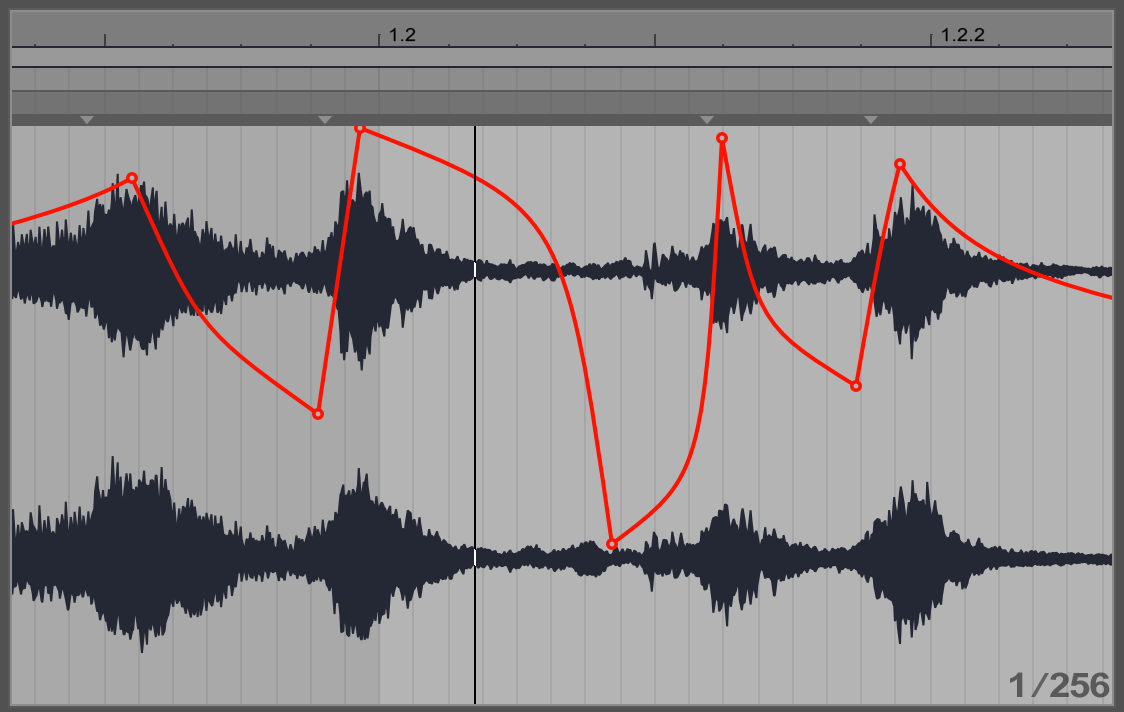
\includegraphics[width=\linewidth]{gfx/03_gesture/AbletonLiveAutomation_72dpi.png}
		\caption{Une courbe d'automation dans le logiciel Ableton Live}
		\label{fig:gesture:automation}
	\end{minipage}
	\hspace{.02\linewidth}
	\begin{minipage}[t]{0.48\textwidth}
	    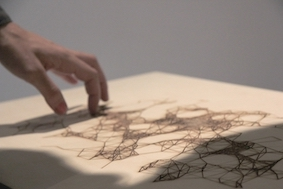
\includegraphics[width=\linewidth]{gfx/03_gesture/EnriqueThomas-TangibleScore_72dpi.jpg}
		\caption{Partition tangible d'Enrique Tomás}
		\label{fig:gesture:tangible_score}
	\end{minipage}
\end{figure}

Stiegler développe le concept de ``gramme'' comme \iquote{corps organisé de signes et de symboles} et emprunte à Sylvain Auroux \cite{auroux_revolution_1994} le concept de ``grammatisation'' comme \iquote{le processus par lequel le continuum temporel des comportements humains est transformé en un spatial discret, qui permet de les intégrer dans les outils}.

Pour Stiegler, les objets sont des enregistrements\footnote{Stiegler utilise les termes de ``rétentions tertiaires'' pour décrire cette inscription de la mémoire dans les objets, afin de la mettre en perspective des ``rétentions primaires'' que sont la conscience du flux temporel et les ``rétentions secondaires'' que sont les souvenirs qui constitue l'expérience d'un individu.}, dans laquelle la mémoire de ce que nous faisons est déposée sous la forme d'une mémoire technique. Ainsi de l'instrument qui incorpore la mémoire du luthier à travers son ergodynamisme, ainsi de la partition qui a enregistré le travail du compositeur\footnote{Jean-Paul Olive parlerait de ``gestes sédimentés'' du compositeur \cite{olive_expression_2013}}.

On voit dans ce concept de ``geste programmé'', la rencontre du travail du luthier et du compositeur qui fait écho à la frontière devenue floue entre ces deux aspect de la création musicale: l'instrument est ``composé''  \cite{schnell_introducing_2002}, la partition est ``instrumentalisée''\footnote{Voir à ce sujet le travail explicite de Enrique Tomás sur les ``partitions tangibles'' \cite{tomas_tangible_2014}}.

\iquote{Quant à la duction de l'instrumentiste, elle vient retemporaliser ce qui ne peut être que spatial : le travail de la composition, ce n'est que spatial, c'est du temps spatialisé, et en cela, essentiellement en défaut d'être. C'est du virtuel pur. C'est du temps discrétisé et détemporalisé dans cette mesure. Discrétisé, il devient manipulable dans sa détemporalisation temporaire telle que la pratique le com­positeur, mais il n'est que virtuel. Il ne peut devenir actuel qu'avec l'interprète, qui doit le re-temporaliser.} B. Stiegler dans \cite{stiegler_circuit_2004}

Cependant, il ne faudrait pas prendre ces ``gestes programmé'' pour de simples enregistrements à repoduire tels quels. La perspective de performance musicale à partir de ces gestes programmé suppose un ``jeu'' avec le geste enregistré, sinon ce ne serait pas un musicien mais, justement, un utilisateur qui démarre, par exemple, la lecture d'un enregistrement audio. La performance musicale consiste justement à faire entendre ce qui n'est pas calculable comme le dit Stiegler \cite{stiegler_circuit_2004}:
 
 \iquote{Un musicien, c'est quelqu'un qui d'abord entend, c'est-à-dire qu'il est primordialement affecté par l'oreille, une oreille qui a cependant des yeux et des mains, et un corps qui les relie. Il ne se contente pas de calculer. Il peut calculer, il doit même calculer, mais s'il le fait, c'est pour donner à entendre ce qu'il a lui-même entendu comme l'incalculable même.}

 Ces gestes programmés ne sont donc pas de simple enregistrements linéaire, mais des modèles complexes et dynamiques qui invitent à des gestes de re-sonnance (voir section suivante) et auxquels la notion de ``modèle intermédiaire dynamique'' (cf. \ref{sec:algorithms:MID}) fait écho.

\textbf{Extra notes}\\

Geste composé (écrit, enregistré, extrait d'analyse, ...) sous forme intensive ou extensive et produit par les machines.\\
Mouvement des machines (cf. Patrick Saint Denis machines mobiles)\\
Mouvement dans l'image (cf. Serge de Laubier musique visuelle => festival, \iquote{amplifier l'écoute par l'image})\\
\iquote{Musique, Incarnation, physique, informatique, voilà quatre fusions de l'alliage dur-doux. (...) Nous nous étonnons devant dces quatre miracles, ces quatre fusions, parce que nous manquons d'une philosophie du mélange} Michel Serres, Musique


%-------------------------------------------
\subsection{Le geste de ré-sonance}

Nous avons vu que le geste musical peut se retrouver incorporé dans le corps de l'instrument sous forme de geste programmé. Ce geste programmé appelle à la mise en mouvement temporelle par le musicien.
Dans le cas de l'instrument acoustique, l'instrument pris isolément est un système passif dont la résonance est purement acoustique : les modes de vibrations propres des corps résonant de l'instruments répondent aux gestes d'excitation et il est possible de modéliser cette résonance acoustique en mesurant la réponse impulsionelle de l'instrument.

Cependant, l'instrument ne joue pas seul et le couple instrument/instrumentiste n'est plus un système passif puisque l'instrumentiste apporte une énergie et vient moduler le son on modifiant 

dans la mesure où l'instrumentiste agit sur les modes acoustiques qui conditionne la durée de vie (ou d'extinction, selon la persepctive adoptée) du son. \\
Dans le cas de l'instrument numérique, le système est actif et le geste de re-sonance est un geste de manipulation interactive du geste\/son programmé.
Il s'agit à la fois de faire sonner ce qui est latent dans le son, mais également de trouver la relation spatio-temporelle d'interaction qui va permettre à l'instrument de sonner comme on le souhaite et de ``jouer'' avec le geste programmé.

Le geste de résonance implique à la fois la chorégraphie du geste et la spectromorphologie du son\footnote{sur la spectromorphologie du son, voir Christopher Small}, dans une relation de correspondance. Cette relation est doublement dynamique, dans la mesure où le geste et le son ont leur propre mouvement interne d'une part, et dans la mesure où ils s'influencent l'un l'autre. Ainsi, la relation de ``résonance du geste'' se construit sur le plan [fonctionnel du geste] instrumental en même temps que sur le plan [métaphorique du geste] musical.

Un exemple significatif est l'interprétation de ``Hangsimogato N°2'' de György Kurtág Jr\footnote{Vidéo disponible sur \url{https://www.youtube.com/watch?v=MJ8Z5skovLw}}. Dans cette pièce, le développement musical se fait par avancement sur une partition pré-programmé par l'intermédiaire d'un capteur Infra-Rouge (D-Beam). Le capteur lui-même n'est pas sensible à l'orientation de la main ou à quelle main (gauche ou droite) vient couper le rayon, mais György Kurtág Jr développe tout un vocabulaire gestuel qui établit des relations de correspondance avec le son. Ces relations de correspondance peut s'appuyer sur une similarité de morphologie énergétique, mais dans certains cas (e.g. geste de présentation des mains ouvertes vers le ciel, replis des bras en croix) elle sont purement métaphoriques et poétiques.

\todo{rajouter un screenshot de la vidéo de Gyorgy}


Le geste de résonance établit un lien



%%%%%%%%%%%%%%%%%%%%%%%%%%%%%%%%%%
\section{Subversion sonore, subversion gestuelle}

\subsection{Définition} 

Le terme ``subversion'' (du latin \textit{subvertere} : renverser, bouleverser) désigne ``l'action visant à saper les valeurs et les institutions établies'' (dictionnaire Larousse). Les moyens employés par la subversion consiste à diffuser un message contraire à un l'ordre établi, dans le but d'affaiblir celui-ci.

Dans le cas de la musique, si la notion de subversion peut prendre une dimension culturelle ou politique dans certains courants musicaux, c'est ici dans le cadre de la perception que j'emploie ce terme.



La subversion peut intervenir à différents niveaux. Au niveau de la composition, l'écriture musicale permet des modulations qui déjouent les attentes de l'auditeur. (e.g. Pink Floyd, breathe transition). Elle peut également se situer au niveau du jeu, en usant de procédés comme des gestes qui contredisent ce qu'on entend et vont l'amplifier. Gyorgy Kurtag Jr. geste violent pour jouer une nuance pianissimo.

Exemples comparés de Applebaum Aphasia et Vincent Carinola/Jean Geoffroy "Rhizome".
BBC Classic Album: "Pink Floyd - The Dark Side of the Moon"

Dissonance cognitive.

Synchrèse de Michel Chion.

Parler du playback, du air-guitar, de la synchrèse.

Bien que ces catégorisations du gestes décrivent adéquatement différents aspects du geste instrumental sur des instruments acoustiques, il semble que le geste musical intègre une aspect subversif souvent négligé.

En particulier, dans le cas des \gls{DMI}, la relation entre le geste et le son est totalement sujette au design de ce que l'on nomme communément le \gls{mapping} et la part de subversion devient partie intégrante du design de ce mapping. 

% Richard Leppert dans \cite{leppert_sight_1993} (cité par \cite{iazzetta_meaning_2000}) souligne à quel point la nature intangible du son et de la musique est polarisée par l'expérience visuelle :
% \begin{quotation}
% Precisely because musical sound is abstract, intangible, and ethereal [...] the visual experience of its production is crucial to both musicians and audience alike for locating and communicating the place of music and musical sound within society and culture. [...] Music, despite its phenomenological sonoric ethereality, is an embodied practice, like dance and theater." 
% \end{quotation}

Il semble dès lors que l'on peut envisager d'autres types de relation entre le geste et le son, afin de tenter de décrire les différents rapports qu'ils entretiennent selon les situations.

Risset fait remarquer l'importance de l'histoire du son d'origine mécanique dans la perception des sons \cite{risset_son_1992}: 

\begin{quotation}
II semble à première vue que l'acoustique numérique puisse s'affranchir de la mécanique. Cependant notre ouïe a évolué dans un environnements d'objets vibrants: aussi la prise en considération des contraintes et des particularités des vibrations mécaniques est-elle importante pour comprendre les idiosyncrasies de la perception auditive et pour en tirer parti.

Les limites de l'acoustique numérique dépendent des capacités différentielles de perception davantage que des contraintes mécaniques. Pourtant, notre perception auditive est orientée par un monde de sons produits mécaniquement, et la mécanique ne doit pas être écartée de façon cavalière, comme l'ont suggéré les travaux de Gibson et Cadoz : les spécificités des vibrations mécaniques mettent en lumière l'organisation perceptuelle dans le processus auditif


\footnote{The limitations of digital acoustics depend upon the differential capacities of perception rather than upon the constraints of mechanics. Yet our auditory perception is geared to a world of mechanically-produced sounds, and mechanics should not be given a cavalier dismissal, as the work of Gibson and Cadoz has suggested : the specifics of mechanical vibrations shed light on the the perceptual organization in the hearing process.} TODO : traduire l'anglais, plus riche.
\end{quotation}


\textbf{Proposition}
\vspace{-1em}
\begin{itemize}[noitemsep]
\item readable gesture to sound relations
\item confusing gesture to sound relations
\end{itemize}

\vspace{-1em}
\begin{itemize}[noitemsep]
\item Gestes emphatique = en phase avec le mouvement interne du son
\item Geste apophatiques = en opposition de phase avec le son
\item Geste unrelated
\end{itemize}

%---- Figure : Einarsson sculpture ---------
\begin{figure}[!htbp]
	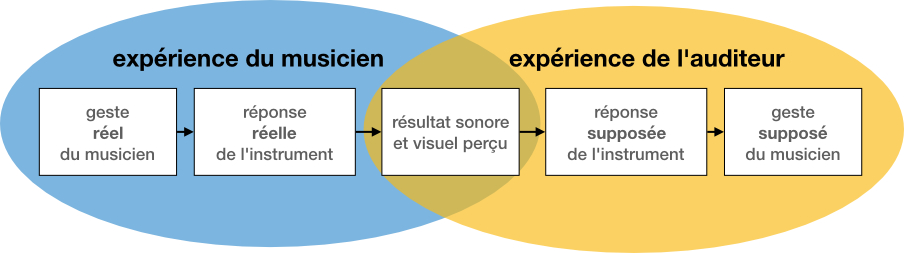
\includegraphics[width=\textwidth]{gfx/03_gesture/gesteReelGesteSuppose.jpg}
	\caption{Geste produit, geste perçu, fonctionnement réel et supposé de l'instrument}
	\label{fig:gesture:RealVsSupposed}
\end{figure}


%-------------------------------------------
\subsection{Continuités artificielles}

\vspace{-1em}
\begin{itemize}[noitemsep]
\item Contrepoint : relier la mélodie à l'harmonie 
\item Bach et le tempérament = relier les différents modes, via la modulation.
\item les doigtés alternatifs, sur le plan gestuel, permettent de sacrifier la justesse de la note, pour établir une continuité gestuelle fluide
\item La musique sérielle : relier la gamme tempérée au spectre en ordonnant 
\item Stravinsky, Russolo : relier l’harmonie et le bruit 
\item jouer un pattern connu ("qu'on a dans les doigts") tout en substituant les notes permet de jouer de manière fluide une mélodie inhabituelle. => numérique
\item Cage, Murray Schaeffer : relier le déterminisme et le hasard, la musique et l’environnement 
\end{itemize}

=> voir Théories de la composition musicale au XXe siècle 
Conjointement à ces explorations compositionnelles se sont développées des techniques et des technologies permettant d’appréhender ces nouveaux espaces. Que cela soit des procédés d’écriture ou des instruments reflétant ces méthodes et modèles.

\subsection{L'importance du format de données}
La possibilité d'établir des continuités entre des espaces gestuels et sonores dépend en partie de la possibilité d'exprimer cette espace dans le format de données adéquat. Par exemple, exprimer une grande polyphonie dont le nombre d'élément est fixe sera probablement plus facilement exprimable à l'aide de matrices, alors que des événements distincts sera plus aisément exprimés sous formes de messages indépendant. De la même manière, des événements déclencheurs peuvent être facilement exprimés sous la forme de messages asynchrones tels que des messages MIDI, mais le flux de ces événements devient très rapide et que leur rythme importe, il sera peut-être plus efficace de les délencher à l'aide d'un signal synchrone tel qu'un signal audio. Cf. Stockhausen Kontakte.


%-------------------------------------------
\subsection{Dans les instruments traditionnels}

%-------------------------------------------
\subsection{Dans les instruments numériques}


Les DMI ont souvent été analysés en tant qu'interface homme-machine, et les conférence académique qui leur sont consacrés reflètent une culture dans lequel l'interaction s'exprime via un cahier des charges préalablement identifié: une interface homme-machine est utilisée dans le cas d'une tâche précise et sa qualité (ergonomie, précision, etc.) peut être mesurée de manière quantifiée.
Dans le cas des instruments de musique cependant, cette tâche est plus complexe, car les enjeux de la création musicale dépassent par essence tout objectif identifié et mesurable au préalable. Par ailleurs, les DMI sont destinés plusieurs types "d'utilisateurs" ayant un rôle différent : le musicien qui joue de l'instrument, mais également le public, qui bien qu'il ne joue pas de l'instrument est amené à en observer la performance.

Low entry fee, high ceiling.

La performance musicale est un "jeu" qui comporte une part de duplicité. Le public d'un concert est toujours le sujet d'une illusion. 

Un des biais de la littérature sur l’affordance des instruments de musique numérique est qu’elle s’inspire souvent des objectifs de l’affordance des HCI en général, avec l’idée que l’instrument doit être compréhensible pour les “autres” utilisateurs potentiels que l’auteur de l’instrument. Pourtant, nombre d’instruments présentés dans la communauté NIME ne sont joués que par leurs auteurs (cf. [1], [2], [3]) et si le fait de vouloir transmettre son instrument aux autres est louable, il n’est pas gage de qualité en ce qui concerne la création qui sera faite avec cet instrument. 


L'art musical procède en partie de la magie et de l'illusion perceptive. Le musicien nous fait entendre des continuités (e.g. une mélodie) là où l'acoustique fait apparaitre une série discrète (e.g. des notes de piano), ou inversement des fissions (e.g. deux voix indépendantes) là où est jouée une série temporelle de notes sur un même instrument. (=> plutôt que des exemple entre parenthèse, mettre une figure illustrant fission e.g. Bach's Violin Partita No. 3, BWV 1006.)

Cette question du jeu entre le continu et le discret dépasse le seul cadre de la musique mais semble trouver dans cet art de nombreuses espaces d'expression.

Les théories de la perception, en particulier du Gestalt, viennent en partie expliquer les mécanismes qui pousse notre perception à créer des continuités où il n'en existe pas physiquement et inversement à catégoriser des événements selon certaines distances perceptives qui ne sont pas nécessairement en lien avec l'unité de source de production du son.

Si donc on analyse le geste musical, il faut nécessairement prendre en compte sa dimension subversive en ce qu'elle se traduit, particulièrement dans le cas des DMIs et des productions musicales impliquant l'électronique en général, dans le design des instruments et outils qui servent à la créer.

\cite{bin_show_2018}

Une étude de Tsay \cite{tsay_sight_2013}, dans laquelle des amateurs et experts sont amenés à évaluer une performance musicale sur la seule base d'un enregistrement silencieux, met en évidence le rôle considérable du la part visuelle dans l'appréciation et l'évaluation de la performance.

Carte et guide , frettage adaptatif (cite \cite{goudard_playing_2014})


Plusieurs articles des NIME analyse les DMI comme \gls{HCI} : 
Louange de la transparence : \cite{fels_mapping_2002}

\iquote{De même, pour un violoniste, la manière dont il lève le bras et dont il va attaquer le son, la rapidité avec laquelle il prépare son coup d’archet nous renseignent un petit peu, mais pas complètement – parce que l’on ne sait pas quelle hauteur il va jouer – sur certaines catégories du son, comme le fait que le son sera agressif, fort, ou délicat et très doux. (...) Dans la musique instrumentale, cette causalité est très importante car cela participe de la façon dont nous la percevons et l’intérêt, avec la musique électronique, c’est que l’on peut remettre en question cette causalité-là : un tout petit geste peut provoquer une tempête. Entre le geste du pianiste qui va appuyer sur une touche du piano et le son qui va sortir, il y a une machine que j’appelle une boîte noire, qui peut inverser les polarités, c’est-à-dire que je peux très bien programmer la machine de manière à ce que plus le son qui va être joué va être minime, pianissimo, plus le son électronique qui va sortir va être au contraire démesuré : dans ce cas-là, le geste ne correspondra pas du tout au son.} Manoury interviewé par Anne-Sylvie Barthel-Calvet. (\url{https://geste.hypotheses.org/364})

Dans en Echo de Manoury, ce sont les formants de la voir qui contrôlent la partie électronique, c'est à dire un geste invisible, sans contact. (extensible au suivi de partition)


%%%%%%%%%%%%%%%%%%%%%%%%%%%%%%%%%%%%%%
\section{Morpho-dynamisme dans les DMI}

Mettre capture d'image du MID qui passe d'une structure rotative à un Verlet.

Comment la continuité s'établit ?



\section{Co-performance}
Ainsi, la nature dynamique et générative des DMIs déplace l'agentivité de l'interaction instrumentale, qui ne saurait être réduite à une relation unidirectionnelle, où le retour haptique et/ou vibratoire n'aurait qu'une dimension épistémique et informative pour le musicien.
L'instrument peut se retrouver en position de mener le jeu et imposer sa cadence à l'instrumentiste. La performance musicale avec un DMI est donc une co-performance où la distribution du contrôle de la synthèse et de la gestuelle qui la provoque, ou en découle, peut se distribuer de manier polymorphe. Une partie de la dynamique de jeu peut être prise en charge par la machine et une autre partie par l'instrumentiste dans une relation qui peut parfois s'approcher d'un duo.

 La performance musicale avec un DMI est donc une co-performance où le contrôle de la synthèse est distribué entre la machine et le musicien. 
 Les gestes du musiciens ne sont ainsi par nécessairement des gestes de contrôle (puisqu'il peuvent être "libérés" de cette fonction là) mais peuvent \textit{découler} de la synthèse opérée par la machine. Les gestes du musicien peuvent alors entretenir des relation de nature différentes :

\vspace{-1em}
\begin{itemize}[noitemsep]
\item une relation d'accompagnement, cohérente ou dissonante;
\item une relation de réaction épidermique;
\item une relation neutre.
\end{itemize}
 


 
\section{Conclusion}
\label{sec:gesture:conclusion}
=> Comment ces aspects influencent le design de l’instrument ?

\section*{extra material}
Notion de vivadi

Part of the excitment in the domain of new digital musical instruments in the 21st century can be attributed to the fact this fact as the musical creativity goes beyond the sound itself and includes the system through which it is performed. A downside of this situation, however, is that the novelty and digital features if the instruments create a sense of discontinuity with tradition , alienation, and lack of understanding by the audience as to what the instrument or the performer is actually doing.
\cite{magnusson_sonic_2019}



\iquote{Si ça se trouve, cette notion que dans quelques années, ``tout sera possible avec la technologie'' fera que cela sera compliqué de créer un mystère entier et profond, parce que les gens du coup diront ``oui, j'en ai entendu parler, maintenant on peut faire ça''.
 J'ai un ami (...) qui a fait voler un espèce de morceau de tulle au dessus des gens avec des principes mécaniques, et beaucoup de gens disaient ``ah oui, c'était incroyable mais je pense que c'était un drône'', alors que pas du tout. Mais je me suis dit, c'est vrai que d'ici quelques années, un objet qui vole tout seul en silence dans l'espace, n'aura plus le même pouvoir de mystère qu'il y a quelques années.} Yann Frish dans \url{https://www.youtube.com/watch?v=5BqHXbQC36M}





Subversion du geste : Kagel et le théâtre musical.
\url{https://geste.hypotheses.org/gemme}

\iquote{Dans le domaine du geste, les outils technologiques peuvent bien sûr jouer un rôle complice, démultipliant les perspectives, inversant les conséquences attendues, décelant l'infime ou captant par méthode statistique tel ou tel paramètre du jeu musical.} 


\iquote{(...) s’approprier à la manière d’un mime les gestualités sonores qui, malgré les indications de la partition, ne peuvent être réellement considérées et donc interprétées que via le prisme de l’écoute.}
P. Jodlowsky, L'INOUI n°1, REVUE DE L'IRCAM, Juin 2006
\url{http://www.pierrejodlowski.fr/site/index.php?post/2011}



\noindent Jakboson (1960) :
\vspace{-1em}
\begin{itemize}[noitemsep]
\item \textbf{expressive function}
\item \textbf{representational function}
\item \textbf{conative function}
\item \textbf{phatic function}
\item \textbf{metalingual function}
\item \textbf{poetic function}
\end{itemize}

\noindent David McNeil : 
\vspace{-1em}
\begin{itemize}[noitemsep]
\item \textbf{Iconics} where the gesture resembles the referent (e.g. describing an action or shape of an object with the hands).
\item \textbf{Metaphorics} where the vehicle (the gesture) relates in one of a number of metaphorical ways to the tenor (non-literal meaning) of the gesture, e.g. indicating a container or conduit for ideas, or a gift of an idea or suggestion (cf. Lakoff et Johnson 1980).
\item \textbf{Beats} where the hand, head, eybrows move roughly in synchrony with the rhythm of often emphatic speech, mark a sequence, or a hiatus such as a change of theme or focus.
\item \textbf{Cohesives} which create a gestalt in gesture space which is coextensive with a spoken utterance or – hierarchically – with its parts.
\item \textbf{Deictics} which may indicate an actual physical position, size, distance or direction, but may also place concepts metaphorically in physical gesture space
\end{itemize}


La mémoire et les gestes:
Leroi Gourhan

\iquote{Quant à l’action relayée (force motrice et transmission), elle domestique pour les utiliser des éléments qui étendent et complètent les effets techniques. Dans ce stade évolué, on n’est plus dans le faire mais dans le faire faire, engagé dans la voie techno-scientifique qui ne garde du geste humain initial que ses épures et en analyse indéfiniment les schèmes.} Michel Guérin, \cite{guerin_philosophie_2018}


\iquote{Les propos des instruments qui nous entourent ne sont pas obligatoirement les nôtres. Ils appartiennent à ceux qui ont fait produire les instruments. Les détourner, c’est se libérer. Les instruments récents sont fascinants parce que, plus que tout autre, ils abritent des virtualités ignorées et parce qu’ils permettent des actions libératrices.} Michel Guérin, \cite{guerin_philosophie_2018}



%%%%%%%%%%%%%%%%%%%%%%%%%%%%%%%%%%%%
\subsection*{types de gestes subversifs}

Si les catégories gestuelles décrites par Cadoz et Wanderley se prêtent à la description des gestes sur un instrument acoustique, elle semble inadaptées ou insuffisantes pour décrire la fonction du geste dans une perspective musicale, en prenant en compte à la fois l'aspect sonore mais également l'aspect scénographique de la performance musicale.

\vspace{-1em}
\begin{itemize}[noitemsep]
\item \textbf{gestes de feintes} : déception de l'attente, mais visible après coup. E.g. dans le football, faire semblant d'aller à droite et envoyer le ballon à gauche, en musique: ommettre le temps fort d'un rythme bien établi, etc. La mécanique du geste est entièrement visible mais a été confuse par un changement innatendu.
\item \textbf{geste magique} : La mécanique du geste reste invisible et la logique causale entre le geste et son résultat reste inexplicable, et sujette à spéculation imaginaires.
\end{itemize}


\subsection*{Le geste de résonance}

Le geste de résonance qui associe à la fois une fonction ergotique (de type modulation) et une fonction épistémique (en cela qu'on cherche le \textbf{sweet spot}). 
\vspace{-1em}
\begin{itemize}[noitemsep]
\item Exemple 1 : résonnance de hauteur dans le fait d'ajuster une modulation pour qu'une organisation harmonique particulière s'ajuste, en particulier dans les jeux subtils de battements qui surviennent lors que l'on est proche d'un ajustement ``parfait'', qui aligne les fréquence et produit une consonnance qui annule les phénomènes de battements à proximité.
\item Exemple 2 dans le cas d'un pad réagissant à la pression et qui contrôlerait un flux rythmique, la possibilité de jouer des accents en n'amplifiant, par la pression, que certains battements du flux rythmique nécessite une action en résonnance avec la période propre du flux rythmique généré automatiquement par la machine.
\item Exemple 3 (alignement) : le DJ qui veut mixer pour enchaîner deux morceaux différents doit à la fois ajuster le rythme (tempo et phase) ainsi que la hauteur (en transposant) du morceau entrant.
\end{itemize}

Le geste de résonance peut donc être continu (cas d'un ajustement de hauteur par exemple) ou rythmique (cas de jeu rythmique en rythme avec la machine).
Dans le cas des instruments acoustique, le seul paramètre du son généré de manière autonome par l'instrument est sa résonance, généralement associée à un paramètre de hauteur et de timbre correspondant aux modes de résonance des matériaux utilisés dans la fabrication des éléments résonants de l'instrument. Dans le cas des instruments électroniques et plus encore, des \glspl{DMI}, l'instrument peut générer de manière autonome toute une phrase musicale, tout un morceau. Le geste vient alors accompagner, de manière plus ou moins interactive, 

\subsection*{geste de production du son et geste d'extinction du son}

Dans les instruments acoustiques, le seul paramètre sonore généré par l'instrument seul est sa résonance.
Si dans les instruments acoustiques, l'extinction du son est une donnée inhérente à leur propriétés physiques (les instruments acoustiques étant des systèmes passifs dans lesquels le son décroit inexorablement et s'éteint s'il n'est pas entretenu), les instruments électriques (dont les instruments électroniques et les \gls{DMI}) nécessitent que le son soit explicitement éteint, que cela soit assuré de manière automatisée, via la programmation de l'instrument, ou par un geste venant commander cette extinction.

Le geste de répétition, qui est explicite chez l'instrumentiste classique, s'il souhaite refaire entendre un passage, et est automatisé dans le concept de boucle.

Geste de spatialisation (cf. Bertrand Merlier, Pierre Couprie), de projection. (qui n'est pas simplement une ``modulation'')

Toutes les composantes du son, de la musique, et de la scénographie sont sujettes à l'invention de gestes, selon ce que le musicien décidera comme d'importance pour sa musique.

\textbf{Différence entre geste effectué et geste capté} : un son électroacoustique, par exemple une figure de ``delta'', pourra ainsi avec un même geste de balaiement de la main, et une même interface de captation (e.g. un simple slider sur une surface multitouch), être déclenchée via un seuillage de l'entrée qui déclenche un sample, être produit de manière continue, via un scrub du sample, pourra avoir son intensité sonore fonction de la vitesse du geste ou pas, etc. On voit que pour un même geste, un même son (échantilloné), et un même capteur, les possibilités de relations entre le geste et le son sont multiples. Le pré-geste hors contact avec l'instrument pourra être capté ou non selon le capteur. (e.g. leap motion)








Partant de l'idée que le geste et la musique sont deux phénomène impliquant le mouvement, je chercherai donc à définir l'intention gestuelle en fonction du rapport qu'il entretient avec le mouvement musical.
On peut dès lors envisager trois attitudes principales :
\vspace{-1em}
\begin{itemize}[noitemsep]
\item \textbf{jouer avec} : en phase avec le mouvement de la musique (geste emphatique), en soutenant par un rythme ou une harmonie complémentaire à ce qui est joué
\item \textbf{jouer contre} : jouer contre le mouvement pour chercher à l'annuler ou le détruire (geste apophatique)
\item \textbf{jouer indifféremment} : sans chercher à être ni contre, ni avec
\end{itemize}

On pourra nuancer cette catégorisation brutale en ajoutant une quatrième catégorie, qui se situerait entre 
le jeu ``avec'' et le jeu ``contre'' qui consiste à jouer en ``interférence'', c'est à dire qui vient infléchir une direction


\iquote{J'appelle  technique un acte traditionnel  efficace  (et  vous  voyez  qu'en  ceci  il  n'est  pas  différent  de  l'acte magique, religieux, symbolique). Il faut qu'il soit traditionnel  et  efficace. Il n'y a pas de technique et pas de transmission, s'il n'y a pas de tradition.} Marcel Mausse, les techniques du corps

Il manque un élément important dans cette considération de la tradition. Pour qu'une tradition soit transmise, il faut que des individus la transmette. Cela peut se faire par la contrainte ou un système doctrinal (e.g. un système religieux), mais en cette absence de coercition physique ou mentale, la tradition sera transmise à la condition que les individus croient en la valeur de cette tradition, c'est à dire qu'il lui accorde de l'importance, c'est à dire qu'il l'aime.


%-------------------------- Figure : Shannon ----------------------------------
\begin{figure}[!htbp]
	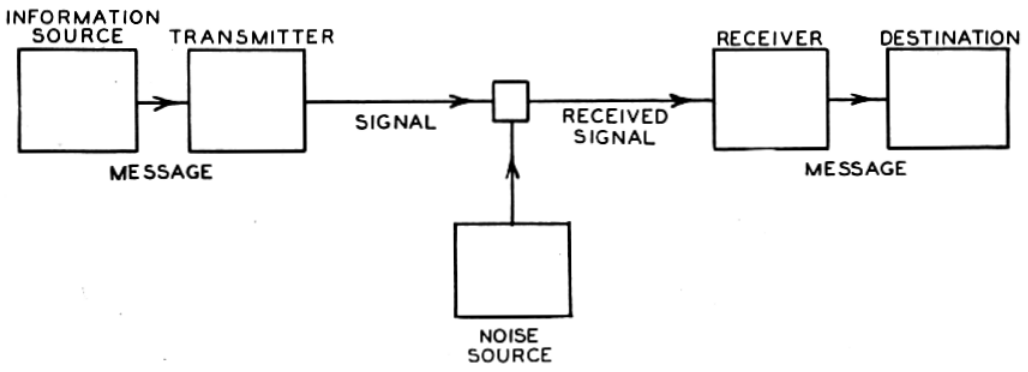
\includegraphics[width=\textwidth]{gfx/03_gesture/ShannonCommunicationSystem.png}
	\caption{Diagramme schématique d'un système général de communication, tel que proposé par Shannon.}
	\label{fig:gesture:shannon}
\end{figure}



Ces deux catégories de geste d'action et de gestes perçu sont emprunt de la théorie de l'information proposée par Shannon \cite{shannon_mathematical_1948} qui envisage la communication comme un système émetteur-message-récepteur unidirectionnel. 
L'inconvenient d'envisager le geste comme simple émetteur d'un signal (qu'il soit travail ou signe) est qu'il empêche de considérer le geste dans la rétroaction dans laquelle il s'inscrit avec l'instrument. En particulier dans la performance musicale, la rétroaction multimodale (par l'ouïe, la vue, le toucher) entre les geste d'un instrumentiste et son instrument, le son et le public est essentielle.








%-------------------------- Figure : transparence Fels -----------------------
\begin{wrapfigure}{R}{0.5\textwidth}
	\begin{center}
 		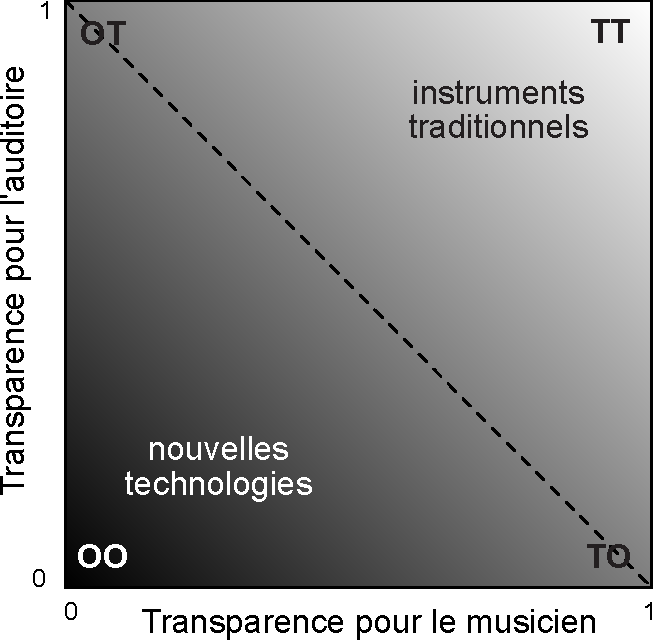
\includegraphics[width=0.48\textwidth]{gfx/03_gesture/Fels-transparency.pdf}
	\end{center}
	\caption{Transparence pour le musicien et l'auditoire, d'après \cite{fels_mapping_2002}}
	\label{fig:gesture:fels_transparency}
\end{wrapfigure}

Certains auteurs ont critiqué cette approche \cite{fyans_where_2009} en remarquant que l'idée selon laquelle une connaissance et une compréhension préalable de l'instrument et de l'idiome était nécessaire pour évaluer une performance musicale, ne pouvait être généralisée aux DMI, à cause de l'émergence rapide de technologies, d'instruments et de pratiques de performance dans ce domaine. 

Cependant, cette critique reste ancrée sur une approche qui considère que le spectateur évalue le \textit{succès} d'une performance selon sa compréhension des intentions de l'instrumentiste.


Le jeu musical joue en partie sur l’attente de l’audience (récompensée ou non) sur la base de règles d'harmonies, d’idiomes (e.g. cadences, résolutions, cycles rythmiques), de citations (e.g. via le sampling), etc..
Affordance des instruments ne peut être réduite aux objectifs d’affordance des HCI.


Kurtag Jr. Hangsimotato (video)
Jean Haury Meta-Piano
Applebaum Aphasia

gestes incongruent (Musical gestures, Godoy, p.48)


Charlotte Moorman and Name June Paik performing John Cage’s 26’1.1499” for a String Player (Human Cello section




%%%%%%%%%%%%%%%%%%%%%%%%%%%%%%

1.Introduction

2.Le geste instrumental défini au tournant du siècle
	2.1 Cadoz, Wanderley
	2.2 Influence de la théorie de la communication

3. Les limites d'une analyse en terme de HCI
	3.1 Geste produit, capté, perçu
	3.2 Les musiciens ne sont pas utilisateurs d'instruments
	3.3 La scène et le laboratoire

4. Du geste instrumental au geste musical
	4.1 L'outil comme externalisation chez L-G
	4.2 Le geste programmé (Stiegler et la grammatisation)
	4.3 Le geste de re-sonance

5. Subversion sonore, subversion gestuelle
	5.1 Sons paradoxaux, gestes paradoxaux
		Risset, Kurtag Jr., Kurtag Père
	5.2 Imaginaire suggéré (cf. texte ci-dessous sur Bayle)
	5.3 Continuité artificielles (morphodynamisme des DMI)
		La musique comme jeu de la (dis)continuité

6. Résonance entre le geste re-sonnant et le son

6. Un exemple pratique 



La notion ``d'image de son (i-son)'' de François Bayle exprime la mécanique psycho-poétique de construction de l'œuvre musicale acousmatique. Sa nomenclature  ne se prête pas facilement à une application directe dans la lutherie (numérique ou non).
En partant de la classification des fonctions de l'écoute proposée par Pierre Schaeffer et Michel Chion (\cite{schaeffer Chion Guide objets sonores page 26}) 

Insérer ici le tableau comprendre-écouter-entendre-ouïr

François Bayle retient notamment trois niveaux d'écoute attentive (en regroupant entendre et comprendre dans un seul niveau) qu'il fait correspondre à trois niveau d'intentionalité dans la mise en jeu des \textit{images-de-sons}:
\vspace{-1em}
\begin{itemize}[noitemsep]
\item \textbf{\textit{im-son}}: l'image isomorphe, iconique, référentielle;
\item \textbf{\textit{di-son}} le diagramme, sélection de contours simplifiés, indiciels ;
\item \textbf{\textit{mé-son}} la métaphore ou métaforme, reliée à une généralité
\end{itemize}

Ces trois catégories font également écho au catégories de Delalande (gestes effecteurs, gestes accompagnateurs, gestes figurés) — sans qu'il y ait toutefois de relations causales triviales entre ces catégories du gestes et de l'écoute.

Romain Bricout : couple ``déclenchement\/modulation'' (analogue à l'archétype ``percussion\/voix'' Martin Laliberté) comme atomes gestuels constitutif de tout mouvement. => NON tout l'espace gestuel avec toutes les connotations possibles (sémiotiques, mimétiques)

Bricout :
\iquote{Déclenchement et modulation représentent donc ces deux gestes primordiaux, à la base de de n'importe quel autre geste plus complexe. Par voie de conséquence, n'importe quel son renvoie lui-même à un geste producteur qui se rapprochera tantôt du déclenchement, tantôt de la modulation ou, par combinaison, des deux à la fois}
=> qu'en est il d'un field recording ?


J'aurais plutôt tendance à employer le terme ``d'image de geste'' (i-geste) pour décrire cette analogie entre les plans d'interprétation du geste et du son.

Le travail de création des correspondances entre geste et son passe ainsi par trois étapes faisant écho à ces différents niveaux de perception/compréhension musicale :
\vspace{-1em}
\begin{itemize}[noitemsep]
\item \textbf{coder} la relation algorithmique (causale ou non), c'est à dire concrètement la relation algorthmique qui s'opère entre les signaux captés par l'interface et le contrôle de la synthèse sonore, 
\item\textbf{jouer} la relation sensible, c'est à dire pratiquer (chorégraphier) l'ensemble du mouvement gestuel dont une partie seulement sera captée par l'interface de jeu;
\item\textbf{imaginer} la relation poétique, cette relation s'établit sur un ensemble plus complexe de valeurs esthétiques, de références culturelles impliquant de manière plus globale les questions de composition, de scénographie, de métaphores portée par les sons, etc.
\end{itemize}



%%%%%%%%%%%%%%%%%%%%%%%%%%%%%%%%%%%%%%%%%%%%%%%%%%%%%%%%%%%%
%%%%%%%%%%%%%%%%%%%%%%%%%%%%%%%%%%%%%%%%%%%%%%%%%%%%%%%%%%%%
%%%%%%%%%%%%%%%%%%%%%%%%%%%%%%%%%%%%%%%%%%%%%%%%%%%%%%%%%%%%
%%%%%%%%%%%%%%%%%%%%%%%%%%%%%%%%%%%%%%%%%%%%%%%%%%%%%%%%%%%%
%%%%%%%%%%%%%%%%%%%%%%%%%%%%%%%%%%%%%%%%%%%%%%%%%%%%%%%%%%%%
%%%%%%%%%%%%%%%%%%%%%%%%%%%%%%%%%%%%%%%%%%%%%%%%%%%%%%%%%%%%
%%%%%%%%%%%%%%%%%%%%%%%%%%%%%%%%%%
\section*{Espace du geste musical}
La musique a longtemps été considéré comme étant faite d'un sous-ensemble de sons, les sons harmonieux, voire harmonique, avant qu'au XXème siècle, les bruits n'y fassent leur place avec les avant-gardes, futuristes. 

John Cage in \cite{cage_silence:_1961}
\begin{quotation}
\noindent If this word, music, is sacred and reserved for eighteenth- and nineteenth-century instruments, we can substitute a more meaningful term: organization of sound.\\
\end{quotation}


Anecdote De Laubier ` le haut parleur ne fonctionne pas'

La musique n'est donc pas faite que de sons, au sens acoustique du terme, mais également (avant tout?) de la perception des sons, qui implique des processus de cognition, des références socio-culturelles, et une sensibilité, une mémoire propre à chacun. 
Ainsi, l'espace de la musique ne se présente non pas comme un sous-ensemble de l'espace des sons, mais probablement comme un sur-espace comprenant à la fois les sons acoustiques mais également tous les liens qu'ils tissent avec notre mémoire.

\Pierre{ voir les 2 définitions de la musique}

L'art musical consiste ainsi à faire entendre des aspects de la musique qui ne sont pas nécessairement présents dans le son, à faire surgir des espaces qui ne peuvent se déployer que dans notre imaginaire, en faisant écho à la trace latente que les sons et la musique ont déjà imprimée en nous.


\begin{quotation}
\noindent Le musical dépasse le sonore en cela qu’il est connecté à une expérience cognitive qui implique la perception et la mémoire.\\
Le sonore dépasse le musical en cela que tout ce qui est sonore ne fait pas nécessairement musique (sauf chez Cage).
\end{quotation}

\Pierre{ ce n'est pas seulement le cas de la musique mais aussi de la parole. Voir définition de Castellengo.}
\Pierre{ Cage -> référence ?}

Là où la présence du musicien sur scène remplissait une nécessité acoustique pour l’écoute, la musique sur support, ou produite par des machines, déplace ce besoin au profit d’une autre fonction, à la fois de compréhension des gestes du musicien (mais est-ce là un jeu de dupes?) et d’un spectacle de l’ordre du funambulisme; le musicien prend des risques [celui de se tromper dans le cas de l’interprétation d’une partition] et la mise en question du corps, réagir au contexte (lieu et au public, ainsi qu’aux éventuels autre musiciens) d’une manière vivante.

L’écoute nous plonge dans des flux sonores, et notre tendance à projeter des causes à ces sons (cf. gestalt) nous emmène sur les lieux — toujours en partie étrangers — de la production de ces flux. sitar indien, crissement de pneu, explosion, acoustique sous-marine ou ambiance de salle de café.
Le musicien crée des passerelles et des agencements entre ces zones liminales.

\Pierre{ si tu parles de gestalt, il faut développer mais c'est aussi une théorie très controversée, donc attention !}

Si les gestes \textit{subversifs} peuvent être assimilés à des gestes accompagnateurs, la plupart des articles de la littérature semble ignorer cette part de subversion au profit de la lisibilité du geste et sa corrélation avec le son \cite{godoy_exploring_2006}.
Cependant, la corrélation n'est pas nécessairement recherchée en tant que telle et si, comme le rappelle Risset, \iquote{la musique est aussi un art du mirage, de l’illusion} \cite{risset_propos_2010}, les œuvres sont nombreuses qui cherchent à dépasser le lien d'apparente causalité entre le geste et le son. 
Il serait alors plus juste d'utiliser le terme de \textit{geste accompagnant la musique}, si toutefois on 

%---- Figure : Einarsson sculpture ---------
\begin{figure}[!htbp]
	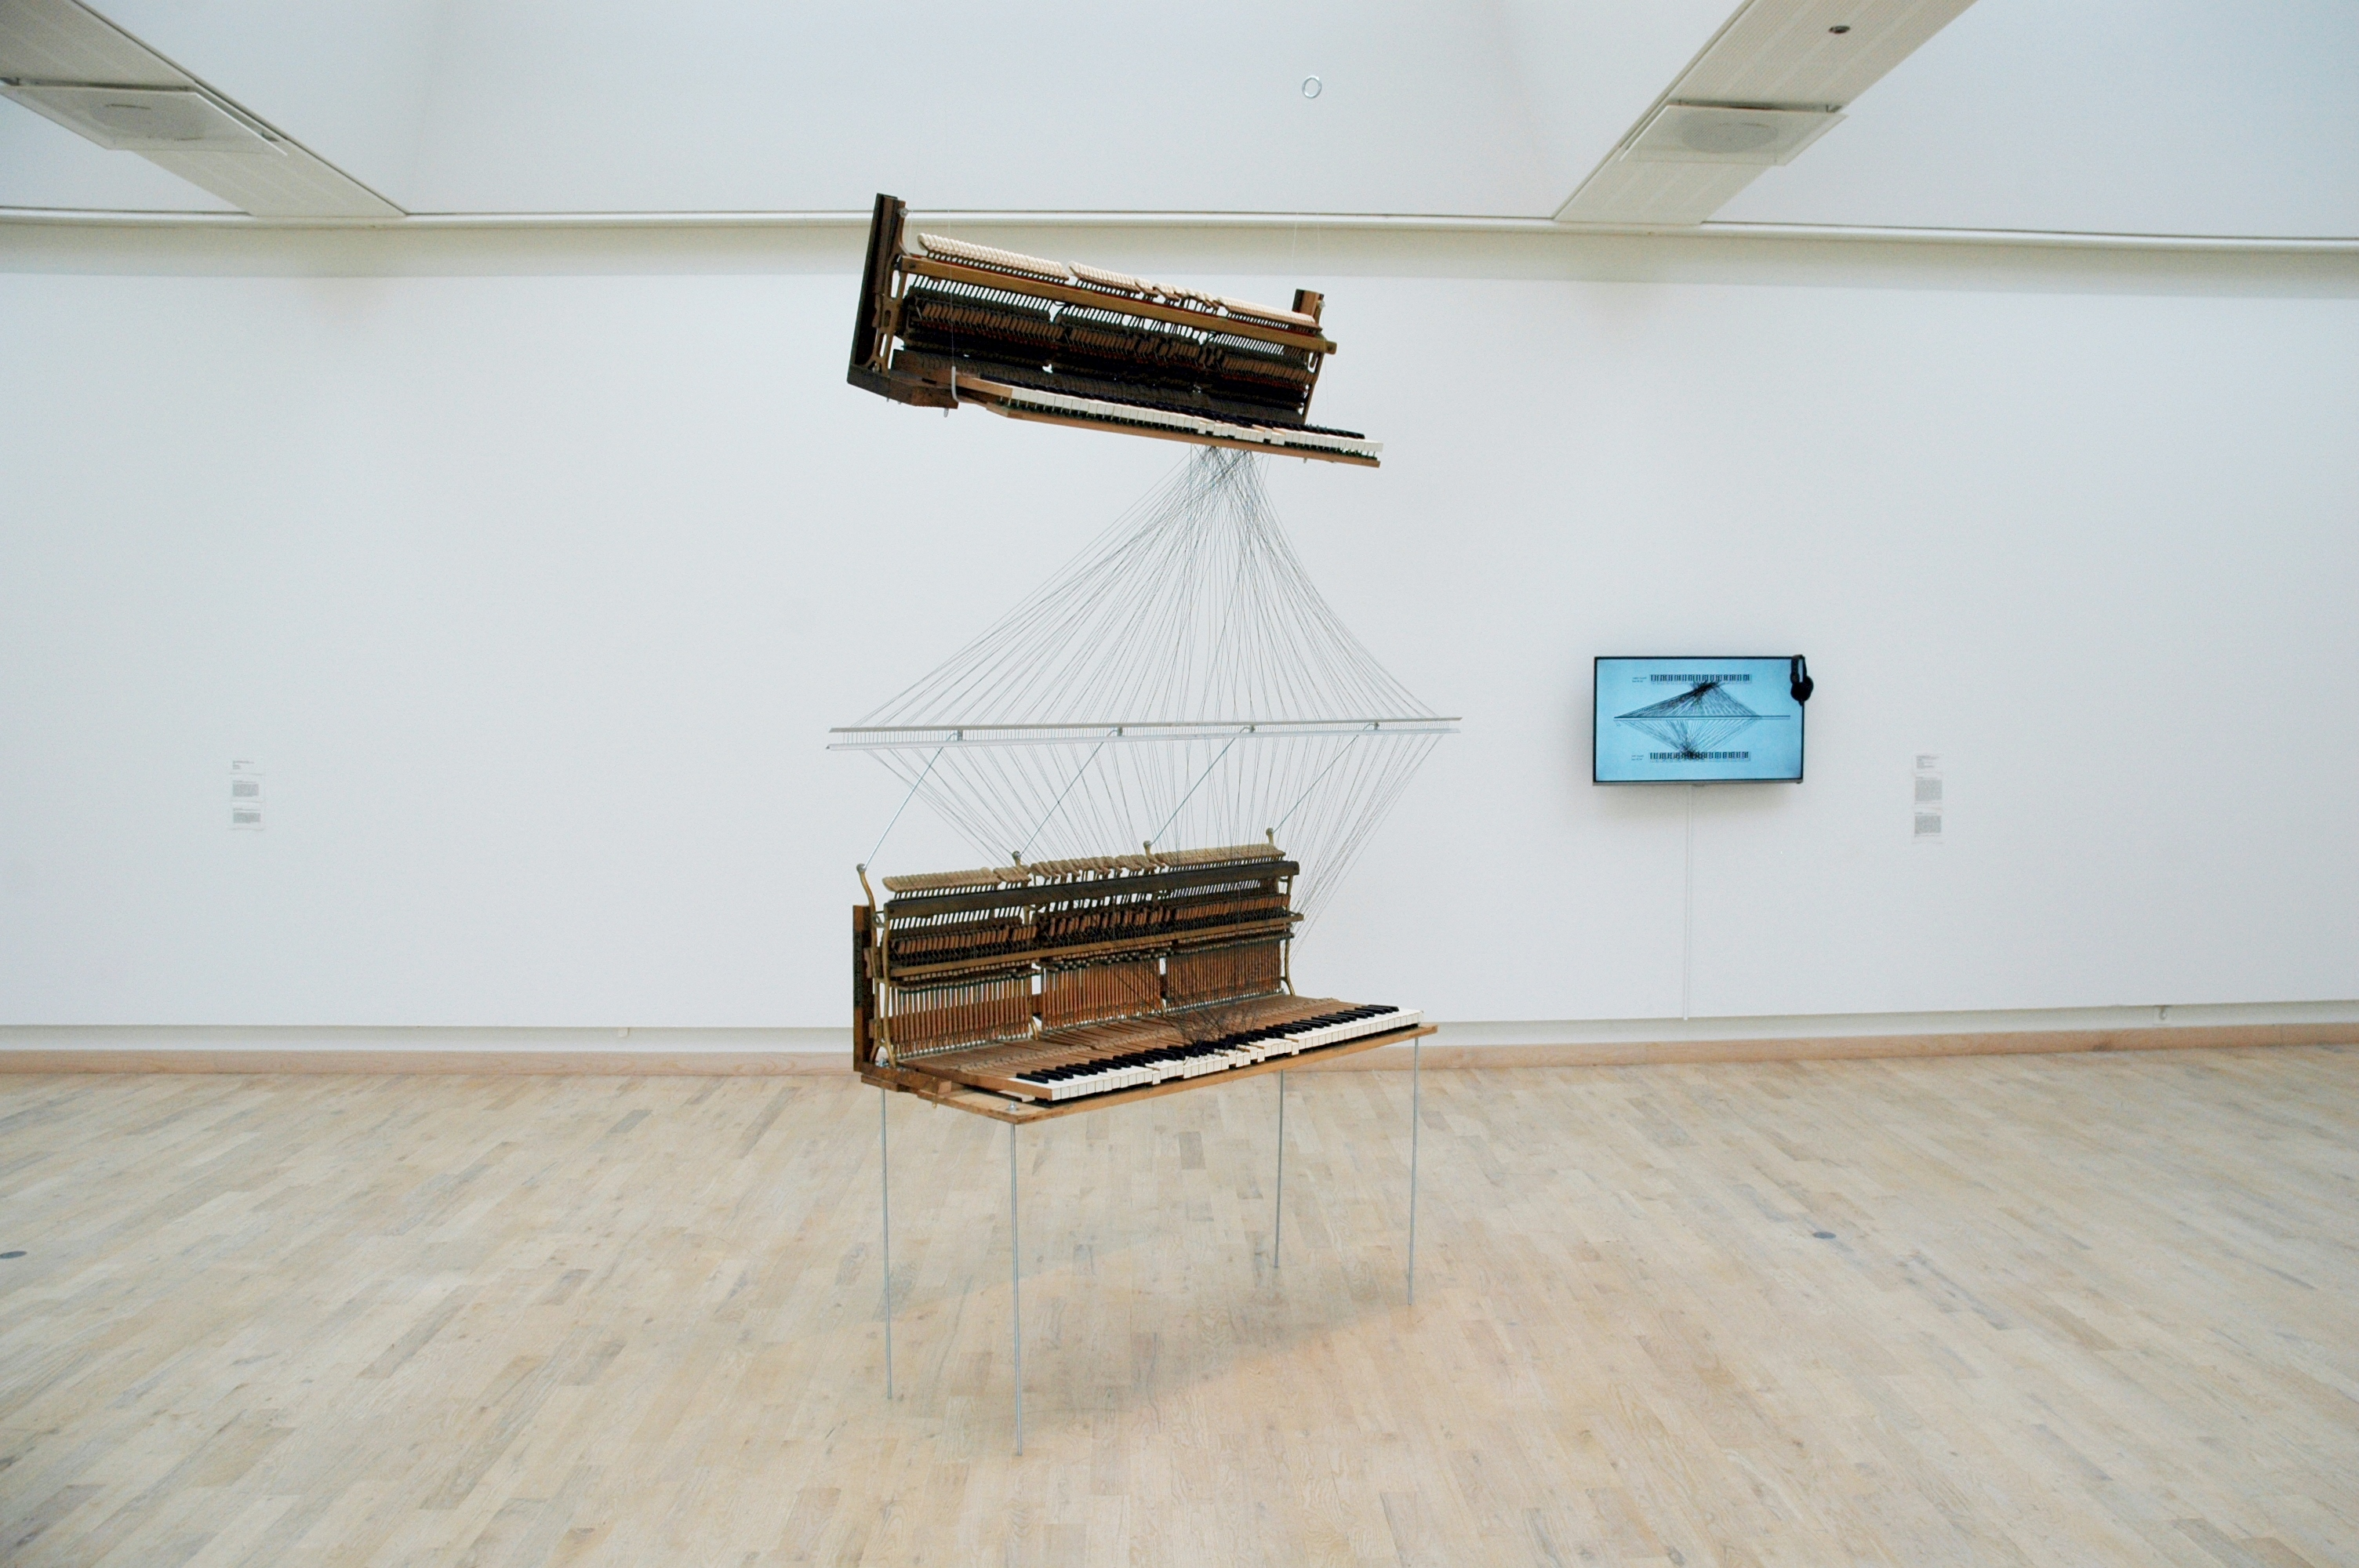
\includegraphics[width=\textwidth]{gfx/Einarson-SchumannSculpture}
	\caption{Einar Torfi Einarsson - Schumann-Sculpture (remnants + deracination)}
	\label{fig:gesture:einarsson}
\end{figure}


\iquote{Every music performance is a dramatic presentation for listeners and improvisers alike. In a sense, both groups play interactive roles as actors from their respective platforms. Just as the design of the hall, the stage and the lighting frames the band's activity for the audience's observation, it also frames the audience's activity for the band to observe. Performers and listeners form a communication loop in which the ction of each continuously affect the other.} Paul F. Berliner in \cite{berliner_thinking_2009}